% Fig. 4 of the QRQT manuscript, standalone for Science Advances.
% Picture copied verbatim from _sciadv_work/drafts_v2/r2.tex (lines 44-160); caption/label are in the main text.
\documentclass[border=2pt]{standalone}
% Minimal preamble shared by the two standalone QRQT figures (Science Advances build).
% Mirrors _sciadv_work/build_v2/nc_main.tex lines 29-62 (only what the pictures use).
\usepackage[T1]{fontenc}
\usepackage{amsmath}
\usepackage{newtxtext,newtxmath}   % Times-compatible, as in the AAAS science_template.tex
\usepackage{xcolor}
\usepackage{tikz}
\usetikzlibrary{calc,arrows.meta,positioning,backgrounds}
% colours used by the two TikZ figures (Fig. 1 and Fig. 4)
\definecolor{classwire}{RGB}{128,0,128}
\definecolor{boxgray}{RGB}{238,240,242}
\definecolor{textdark}{RGB}{48,54,60}
\definecolor{bellfill}{RGB}{220,231,223}
\definecolor{bellborder}{RGB}{122,145,130}
\definecolor{pqcfill}{RGB}{226,232,244}
\definecolor{pqcborder}{RGB}{96,118,156}
\definecolor{pqctext}{RGB}{78,100,138}
\definecolor{advcol}{RGB}{91,128,134}
\begin{document}
\begingroup % TikZ text at the sizes of the 10 pt APS layout the figure was drawn for
\renewcommand{\tiny}{\fontsize{5}{6}\selectfont}%
\renewcommand{\scriptsize}{\fontsize{7}{8}\selectfont}%
\renewcommand{\footnotesize}{\fontsize{8}{9.5}\selectfont}%
\renewcommand{\small}{\fontsize{9}{11}\selectfont}%
\renewcommand{\normalsize}{\fontsize{10}{12}\selectfont}%
\renewcommand{\large}{\fontsize{12}{14}\selectfont}%
\normalsize
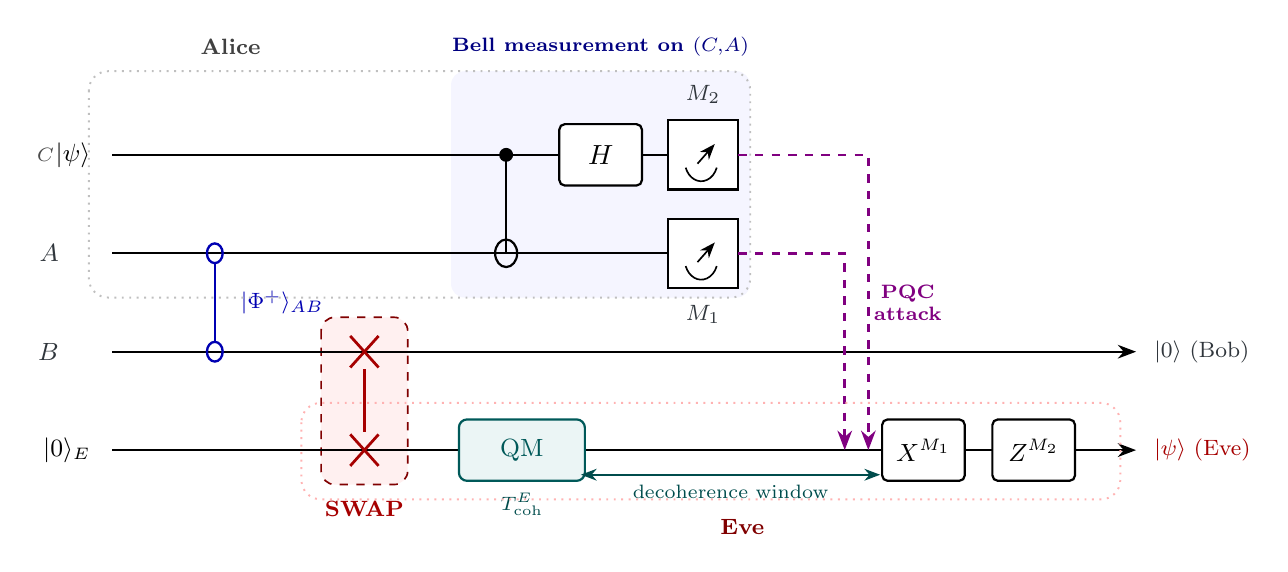
\begin{tikzpicture}[
    x=1cm,
    y=1.25cm,
    >=Stealth,
    thick,
    gate/.style={
        draw, rounded corners=2pt,
        minimum width=1.05cm, minimum height=0.78cm,
        fill=white, inner sep=2pt, font=\normalsize
    },
    membox/.style={
        draw=teal!70!black, rounded corners=3pt,
        minimum width=1.6cm, minimum height=0.78cm,
        fill=teal!8, inner sep=2pt, font=\small,
        text=teal!70!black
    },
    meas/.style={
        draw, minimum width=0.88cm, minimum height=0.88cm,
        fill=white
    }
]

\node[anchor=east, font=\small] at (-0.15, 3)   {$|\psi\rangle$};
\node[anchor=east, font=\small, text=textdark] at (-0.55, 2) {$A$};
\node[anchor=east, font=\small, text=textdark] at (-0.55, 1) {$B$};
\node[anchor=east, font=\small] at (-0.15, 0)   {$|0\rangle_E$};

\node[font=\scriptsize, text=gray!60!black] at (-0.85, 3) {$C$};

\draw[black, line width=0.8pt] (0, 3) -- (8.0, 3);
\draw[black, line width=0.8pt] (0, 2) -- (8.0, 2);
\draw[black, line width=0.8pt] (0, 1) -- (12.6, 1);
\draw[black, line width=0.8pt] (0, 0) -- (12.6, 0);

\draw[blue!70!black, line width=0.85pt] (1.3, 2) circle (0.10);
\draw[blue!70!black, line width=0.85pt] (1.3, 1) circle (0.10);
\draw[blue!70!black, line width=0.85pt] (1.3, 1.90) -- (1.3, 1.10);
\node[blue!70!black, font=\footnotesize, anchor=west] at (1.5, 1.50)
    {$|\Phi^+\rangle_{AB}$};

\begin{scope}[on background layer]
    \fill[red!6, rounded corners=5pt]
        (2.65, 1.35) rectangle (3.75, -0.35);
    \draw[red!50!black, rounded corners=5pt,
        line width=0.6pt, dashed]
        (2.65, 1.35) rectangle (3.75, -0.35);
\end{scope}
\draw[red!65!black, line width=1pt] (3.02, 1.16) -- (3.38, 0.84);
\draw[red!65!black, line width=1pt] (3.38, 1.16) -- (3.02, 0.84);
\draw[red!65!black, line width=1pt] (3.02, 0.16) -- (3.38,-0.16);
\draw[red!65!black, line width=1pt] (3.38, 0.16) -- (3.02,-0.16);
\draw[red!65!black, line width=0.8pt] (3.20, 0.82) -- (3.20, 0.18);
\node[font=\footnotesize\bfseries, text=red!65!black]
    at (3.20, -0.60) {SWAP};

\node[membox] (qmem) at (5.2, 0) {QM};
\node[font=\scriptsize, text=teal!60!black, align=center] at (5.2, -0.55)
    {$T^{E}_{\mathrm{coh}}$};

\begin{scope}[on background layer]
    \fill[blue!4, rounded corners=5pt]
        (4.3, 3.85) rectangle (8.1, 1.55);
\end{scope}
\node[blue!50!black, font=\scriptsize\bfseries] at (6.2, 4.10)
    {Bell measurement on $(C,\!A)$};

\filldraw[black] (5.0, 3) circle (2.1pt);
\draw[black, line width=0.8pt] (5.0, 3) -- (5.0, 2);
\draw[black, line width=0.8pt] (5.0, 2) circle (0.14);

\node[gate] (H) at (6.2, 3) {$H$};

\node[meas] (M2box) at (7.5, 3) {};
\node[meas] (M1box) at (7.5, 2) {};
\draw[line width=0.6pt] (7.28, 2.87)
    arc[start angle=200, end angle=340, radius=0.21];
\draw[->, line width=0.6pt] (7.43, 2.91) -- (7.65, 3.11);
\draw[line width=0.6pt] (7.28, 1.87)
    arc[start angle=200, end angle=340, radius=0.21];
\draw[->, line width=0.6pt] (7.43, 1.91) -- (7.65, 2.11);
\node[above=2pt, font=\footnotesize, text=textdark]
    at (M2box.north) {$M_2$};
\node[below=2pt, font=\footnotesize, text=textdark]
    at (M1box.south) {$M_1$};

\draw[classwire, dashed, line width=0.9pt, ->]
    (7.95, 3.0) -- (9.6, 3.0) -- (9.6, 0);
\draw[classwire, dashed, line width=0.9pt, ->]
    (7.95, 2.0) -- (9.3, 2.0) -- (9.3, 0);
\node[text=classwire, font=\scriptsize\bfseries, align=center]
    at (10.1, 1.5) {PQC\\attack};

\node[gate, font=\small] (Xcorr) at (10.3, 0) {$X^{M_1}$};
\node[gate, font=\small] (Zcorr) at (11.7, 0) {$Z^{M_2}$};

\draw[->, black, line width=0.8pt] (12.6, 1) -- (13.0, 1);
\node[anchor=west, font=\footnotesize, text=textdark]
    at (13.1, 1) {$|0\rangle$ (Bob)};
\draw[->, black, line width=0.8pt] (12.23, 0) -- (13.0, 0);
\node[anchor=west, font=\footnotesize, text=red!65!black]
    at (13.1, 0) {$|\psi\rangle$ (Eve)};

\draw[gray!50, dotted, rounded corners=7pt, line width=0.7pt]
    (-0.3, 3.85) rectangle (8.1, 1.55);
\node[gray!50!black, font=\footnotesize\bfseries] at (1.5, 4.10) {Alice};

\draw[red!30, dotted, rounded corners=7pt, line width=0.7pt]
    (2.4, 0.48) rectangle (12.8, -0.50);
\node[red!50!black, font=\footnotesize\bfseries]
    at (8.0, -0.78) {Eve};

\draw[teal!60!black, <->, line width=0.6pt]
    (5.95, -0.25) -- (9.75, -0.25);
\node[font=\scriptsize, text=teal!60!black] at (7.85, -0.42)
    {decoherence window};

\end{tikzpicture}
\endgroup
\end{document}
